\part{Second Part}
\label{partII}

% \chapter{Contribution}

% You may also put some code snippet (which is NOT float by default), eg: \cref{lst:random-code}.

% \lstinputlisting[float,language=Java,label={lst:random-code}]{listings/HelloWorld.java}
% \label{lst:random-code}

% \cref{lst:metrics-code}.

% \lstinputlisting[float,language=python,label={lst:metrics-code}]{listings/metrics.py}
% \section{Fancy formulas here}

\chapter{Introduction}

% We are witnessing an ever-increasing trend in data production, thus leading to the so-called \emph{Big Data} era. 
% \note[Luca][notesyellow]{Espandere descrizione con esempi e brevi cenni storici}

In the last twenty years, we have witnessed an unprecedented and ever-increasing trend in data production. 
\citeA{hilbert2011world} date the rise of this phenomenon back to 2002, with the beginning of the digital age.
Indeed, the transition from analog to digital storage devices enormously expanded the capacity of accumulating data, thus leading to the \emph{Big Data} era.

The term big data was first introduced in 1990s \cite{16, 17} and it is commonly adopted to describe datasets whose size exceeds the potential to manipulate and analyze them within reasonable time limits \cite{snijders2012big}.
However, the expression does not target any specific storage size but rather assumes a deeper meaning that goes well beyond the sheer amount of data points.
In fact, big data embrace a broad spectrum of data sources including structured, semi-structured and, mostly, unstructured data \cite{dedic2016towards}.
Although multiple connotations have been attributed to the concept of big data over the years, a commonly shared definition is related to the so-called \emph{5 Vs} \cite{3}:

\begin{itemize}
    \item \textbf{Volume}: the actual quantity of generated data is huge, in the order of magnitude of terabytes and petabytes \cite{sagiroglu2013big}. More generally, it indicates amounts that are too large and complex to exploit conventional data storage and processing technologies;
    
    \item \textbf{Variety}: the data may come in several data types and from diverse origins. These include sources as sensors, social media, log files and more, plus they encompass heterogeneous formats like text, images, audio, video and so on; 
    
    \item \textbf{Velocity}: data are produced and/or processed at high rates \cite{kitchin2016makes}, typically nearly real-time;
    
    \item \textbf{Value}: data must carry valuable information that, if correctly analyzed, bring business value and profitable insights \cite{uddin2014seven}. In a scientific context, this means information that contribute to the advancement of human knowledge;
    
    \item \textbf{Veracity}: data sources must be reliable and generate high-quality data that can produce value \cite{onay2018review, 33};


\end{itemize}


Nonetheless, the community has not reached a complete agreement on the big data definition \cite{22, kitchin2016makes}, with some authors suggesting moving their characterization from the intrinsic properties to the techniques adopted to acquire, store, share and analyze the data \cite{balazka2020big}.


Besides the modification of the storage supply,  multiple factors significantly enhanced data production and, hence, favored the rise of the big data era.
% the demand for storage space and computing power.
In the first place, the diffusion of the internet and the progress of computer technologies provided more processing capabilities and easier access to data, thus stimulating further their production.
Consequently, several stakeholders as big tech companies, traditional industries, governments, healthcare institutions and more started increasingly contributing to this growth.
Finally, the introduction of \emph{smart} everyday objects that not only receive but also produce data exponentially accentuated individual contributions to the total data produced.
Modern objects, in fact, are endowed with technologies that allow to collect data and share them via a network -- the so-called Internet of Things \cite{ashton2009iot} --, thus augmenting the production rate even more.
For instance, sensors measuring the status and operation are now commonly used in industrial machinery and household appliances to ease their control and automate maintenance.
The same paradigm is also influencing the direction of the personal items market in various ways.
% and, in turn, new use-cases emerge from their adoption. 
For example, some tech companies are recently investing in wearable devices like watches and glasses to enable the users to be always connected with a rapidly mutable environment, track their progress and explore the world in unparalleled manners thanks to virtual reality.
Furthermore, the solutions that digitization offers are being explored to respond to the emerging challenges of current times.
Think, for instance, of the urge for modernization of institutional processes posed by the pandemic. The massive spread of the infections has required unprecedented amounts of patients needing access to health assistance. However, the impossibility to scale up services and equipment correspondingly caused huge issues and jeopardized people's safety. In such context, the availability of intelligent systems capable of remotely monitoring patients' conditions and providing them with specialist support would have enormously helped.

In order to cope with the growing amount of data to store and process, the big data players of both industry and academy have gradually moved to new computing paradigms in recent years. 
For instance, new solutions as \textbf{distributed} and \textbf{cloud computing} \cite{kshemkalyani2011distributed, wang2010cloud} have been specifically designed to address these new requirements, taking advantage of multiple resources geographically displaced and accessible via a network.

However, the boost in performance guaranteed by these technologies comes with the price of requiring very complex interactions of both hardware and software components. 
Aside from the enormous benefits these solutions bring, their most relevant drawback is that the wider the infrastructure, the higher the chances of something going wrong, and the bigger the effort to detect, inspect and solve the issues.
\Cref{partII} explores this domain and tries to propose a data-driven pipeline to ease and support people working to maintain the infrastructure integrity.
Despite applying to many different applications with some tuning, the presented approach is discussed in the context of \textbf{data transfer failures} within the \emph{Worldwide Large Hadron Collider Computing Grid} (WLCG).
    \section{Background}
\begin{figure}
    \centering
    \subfloat[LHC accelerator]{
    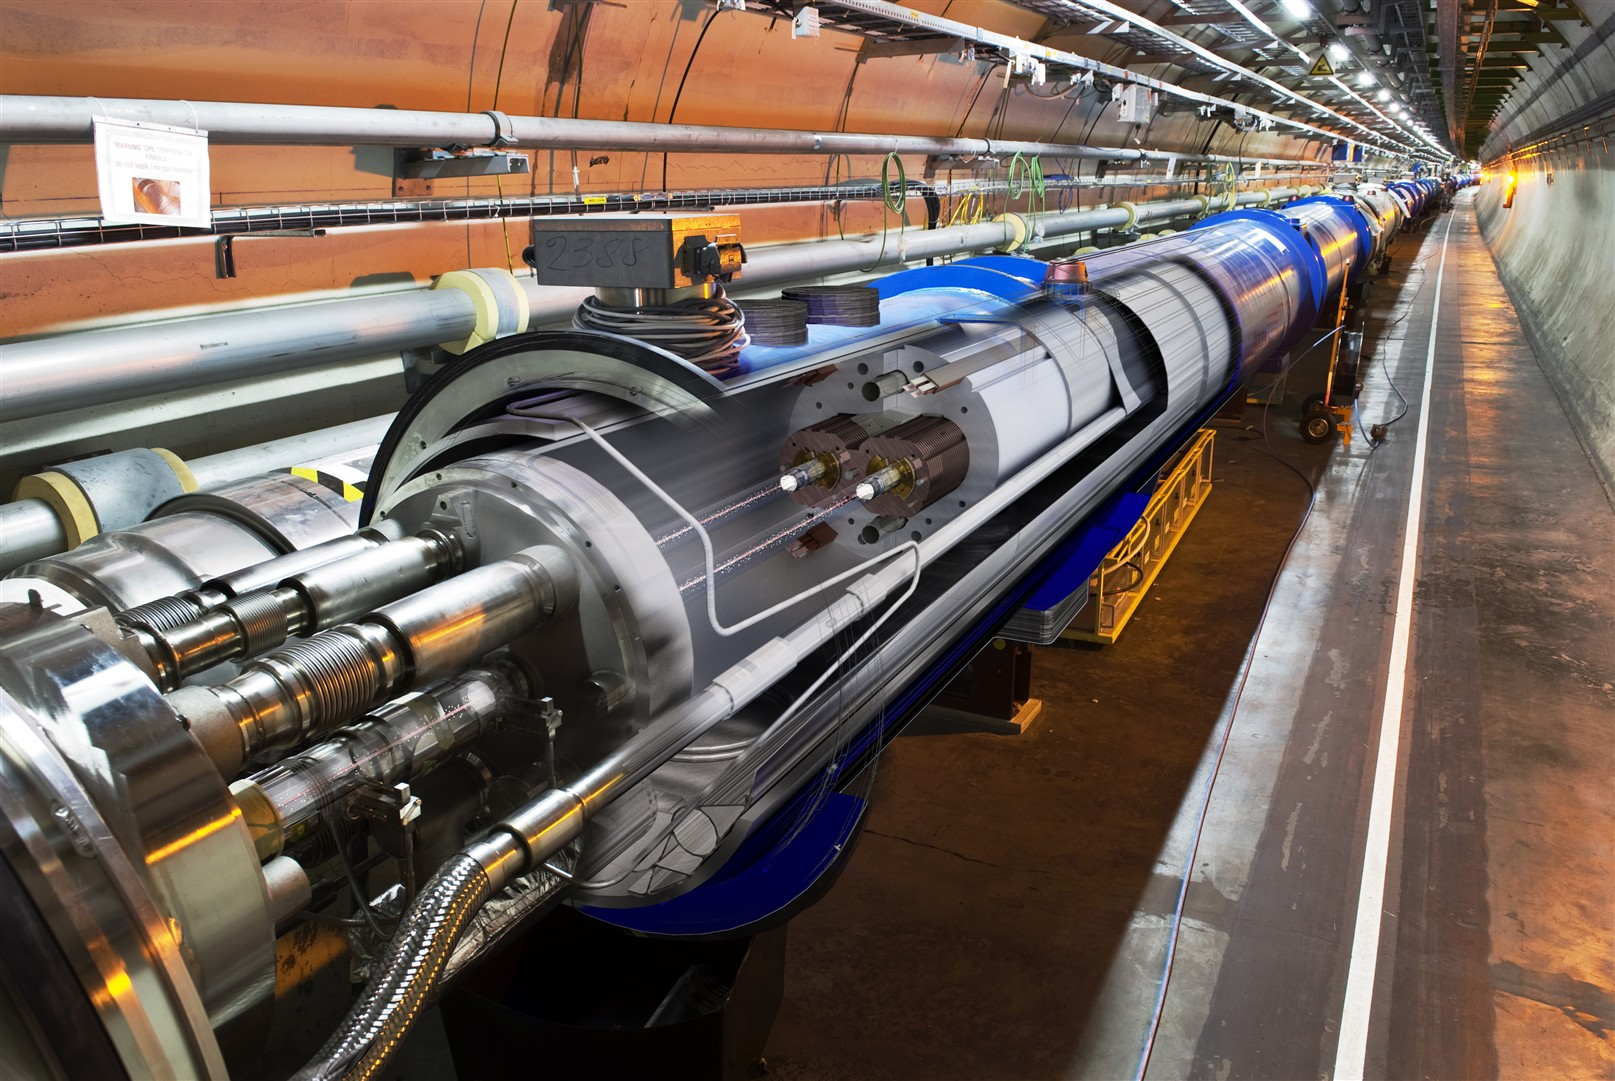
\includegraphics[width=\textwidth]{figures/220_introduction/cern/a0lhcinternotubo_445034351.jpg}
    }
    
    \subfloat[Aerial view]{
    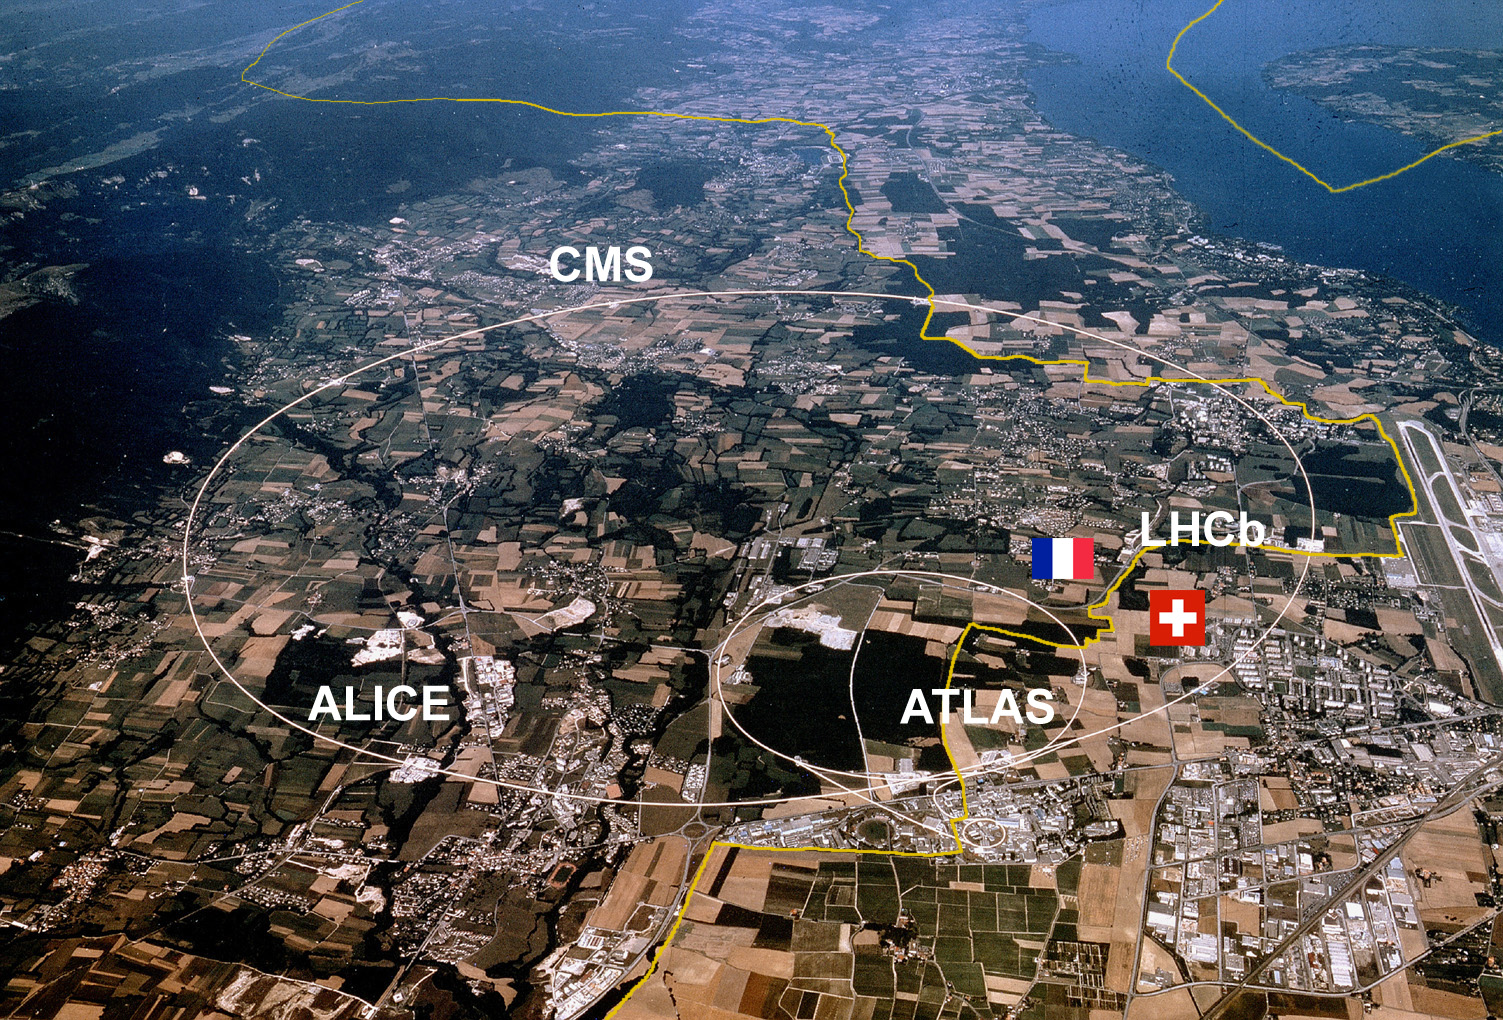
\includegraphics[width=0.5\textwidth]{figures/220_introduction/cern/CERN_location.jpg}
    }
    \subfloat[LHC scheme]{
    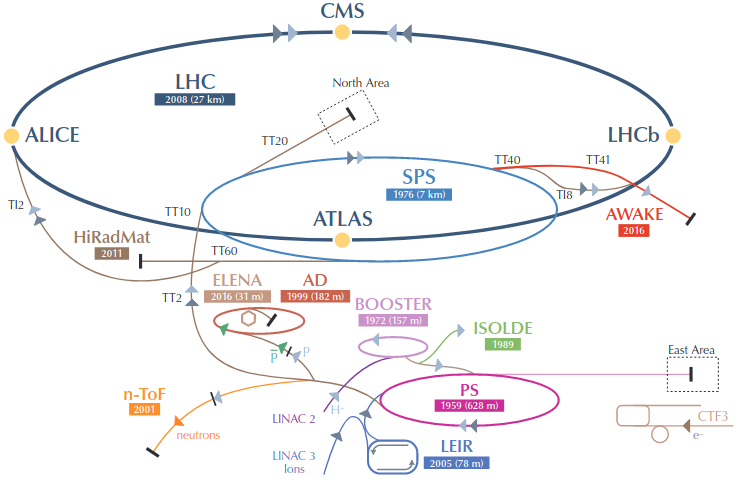
\includegraphics[width=0.5\textwidth]{figures/220_introduction/cern/lhc_scheme_factsfigures.png}
    }
    \caption{\textbf{LHC accelerator complex.} Top: the underground tunnel that hosts LHC and a transversal section of the pipes that compose it. 
    Bottom: aerial view of LHC complex at the boundary between Switzerland and France (left) and structure of the various accelerating structures that compose LHC (right).
    }
    \label{fig:lhc}
\end{figure}

\begin{figure}
    \centering
    \subfloat[ATLAS]{
    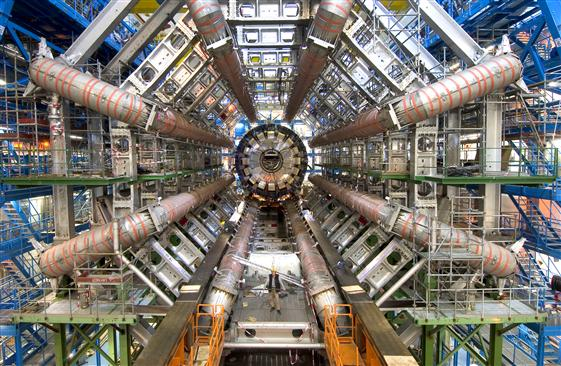
\includegraphics[width=0.5\textwidth]{figures/220_introduction/cern/atlas_detector_medium.jpg}
    }
    \subfloat[LHCb]{
    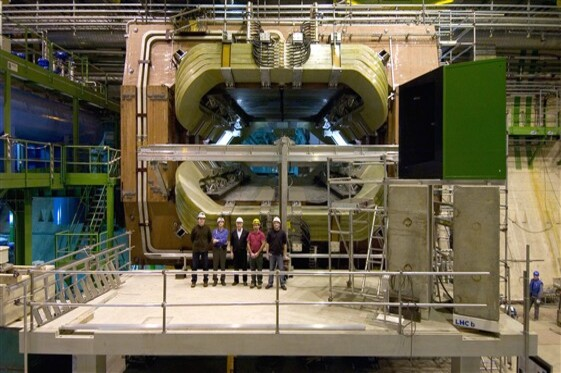
\includegraphics[width=0.5\textwidth]{figures/220_introduction/cern/lhcb_detector_medium.jpg}
    }
    
    \subfloat[ALICE]{
    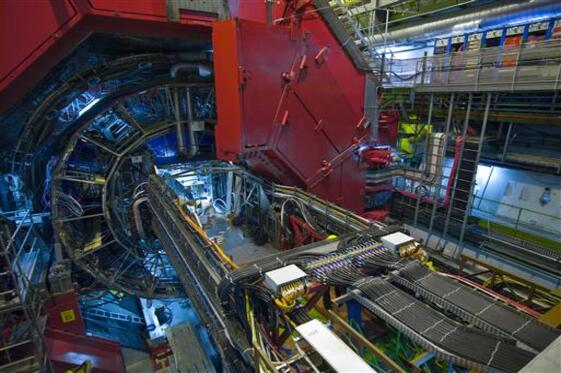
\includegraphics[width=0.5\textwidth]{figures/220_introduction/cern/alice_detector_medium1.jpg}
    }
    \subfloat[CMS]{
    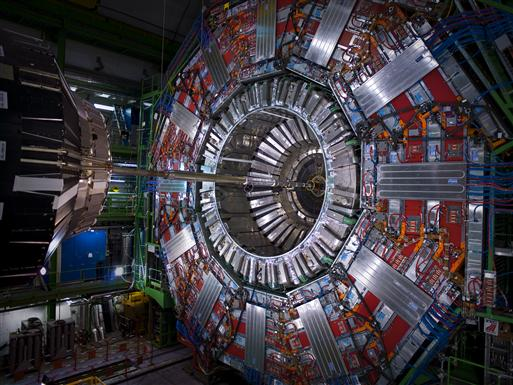
\includegraphics[width=0.5\textwidth]{figures/220_introduction/cern/cms_detector_medium.jpg}
    }
    \caption{\textbf{CERN 4 major experiments.}}
    \label{fig:cern_experiments}
\end{figure}

\note[Luca][notesyellow]{Introduction to HEP community, with mention to WLCG as an essential tool to perform their research}

% High-Energy Physics (HEP) is a branch of physics that studies the fundamental constituents of matter and the forces that drive their interactions. One of the methods is to create very high energy densities. 
% This reproduces the environmental conditions of the primordial universe.

High-Energy Physics (HEP) is a branch of physics that studies the elementary constituents of matter and the fundamental principles that govern their interaction to understand how our universe has formed and evolved.  
These particles, however, are not visible at the scales whereby we experience reality today. 
Thus, HEP experiments need to either look at natural phenomena generated in pressure and temperature conditions similar to those of the primordial universe -- like cosmic rays -- or recreate such settings artificially.

The European Council for Nuclear Research (CERN) is part of this second strand of experiments, and it constitutes the largest particle physics laboratory in the world.
From 2008, CERN facilities also include the Large Hadron Collider (LHC), the longest particle accelerator ever built.
LHC consists of a \mbox{26.7-kilometer} ring located in a tunnel about 100 meters underground in the Geneva area (\cref{fig:lhc}), and it is made of superconducting magnets with several accelerating structures \cite{lhcwebsite}.
Inside the accelerator, bunches of protons are revved up to nearly the speed of light, forming two high-energy particle beams that travel in opposite directions inside separated pipes. 
When they acquire the desired energy, the beams are directed towards dedicated interaction points where the experiments occur. %surrounded by giant detectors.
In practice, LHC hosts four major experiments built in correspondence of these locations -- ATLAS \cite{aad2008atlas}, ALICE \cite{aamodt2008alice}, LHCb \cite{alves2008lhcb} and CMS \cite{collaboration2008cms} -- and equipped with giant detectors (\cref{fig:cern_experiments}).
Once the beams get there, the two pipes cross and the particles are squeezed through substantial magnetic fields to increase their chances of colliding. 
In this way, a massive amount of energy is concentrated in an extremely tiny area, generating millions of particles at each collision.
Indeed, the high speed of the beams causes roughly 40 million crossings per second at each interaction point \cite{albrecht2019roadmap, grandi2017HEPsize}. 
\sidenote[Luca][notesyellow]{Controllare numeriche ed aggiungere reference}
When a crossing happens, an average of 60 bunch collisions -- also referred to as pileup -- are observed \cite{albrecht2019roadmap}. The particles produced by each scattering then fly around the interaction point to be eventually detected through high-technology experimental devices endowed with over 100 million electronic channels \cite{grandi2017HEPsize, aad2020channels}.
According to the latest experimental setup, this delivers 100 MegaBytes (MB) of data per collision and it would generate 40k ExaBytes (EB) every year \cite{grandi2017HEPsize}.
However, storing such a tremendous amount of data is unattainable with current technology and budget. In addition, the events of interest are typically rare, so there is actually no need to record all of the information detected by the electronic channels.
Thus, the vast majority of \emph{read-out} data from collisions is discarded straight away and the \emph{recorded} event rate is lowered to 1k crossings per second. 
As a result of this reduction, the actual acquisition rate
% amounts to 1MB every second, translating to roughly 100 PetaBytes (PB) a year in 2018 \cite{grandi2017HEPsize, altre?}.
amounts to nearly 1 PB per day \cite{cern2017storage}, translating to roughly 160 PetaBytes (PB)%
\footnote{LHC registered 161 days of physics data taking in 2018 \cite{todd2018lhcAvail}}
a year in 2018. %\cite{grandi2017HEPsize, cern2017datayear}.
Besides that, physics analyses require comparing experimental results with Monte Carlo data simulated according to current theories, thus producing somewhat between 1 and 2 times additional data \cite{grandi2017HEPsize}.
Furthermore, the CERN community is already working at enhancing the Large Hadron Collider capabilities.
The project involves boosting the energy of the beam and gradually increasing the pileup towards 200 collisions per bunch crossing \cite{albrecht2019roadmap}, thus leading to the so-called High Luminosity LHC (HL-LHC) \cite{hllhc}.
% Thanks to this upgrade, way more events will be observed as the beam energy will be boosted and the pileup will gradually be increased towards 150 collisions per bunch crossing.
% In this new regime, 
Thanks to this upgrade, the observed events are expected to increase of a factor $\geq5$\cite{hllhc} and produce an estimated 800 PB of new data each year by 2026.%\cite{grandi2017HEPsize, HLLHC_data}.

Although it is difficult to replicate such a punctual measurement of the data production for other big data players, some hints can be retrieved by comparing multiple online resources. %\cite{BDPlot_series}. 
\Cref{fig:bidata_size} tries to summarize a reasonable, up-to-date ``guesstimate"%
\footnote{These data are reconstructed based on multiple online sources about the amount of contents produced, streamed or hosted by big data companies and reasonable estimates of unitary sizes for such contents, e.g. average mail or picture size, average data traffic for 1 hour video, and so on. 
However, the actual values reported are not meant to be extremely accurate and only serve the purpose of giving an idea of the orders of magnitude of the various phenomena.
}
of yearly data production for the main big data companies.
Despite not being the most popular among the mainstream audience, the HEP community is one of the most prominent players concerning big data.
% \begin{landscape}
% \begin{figure}
%     \centering
% \begin{tikzpicture}%[shorten >=1pt,node distance=1cm,on grid,auto] 
% \linespread{.5}%
% \begin{scope}
%     \node[anchor=south west,inner sep=0] (image) at (0,0){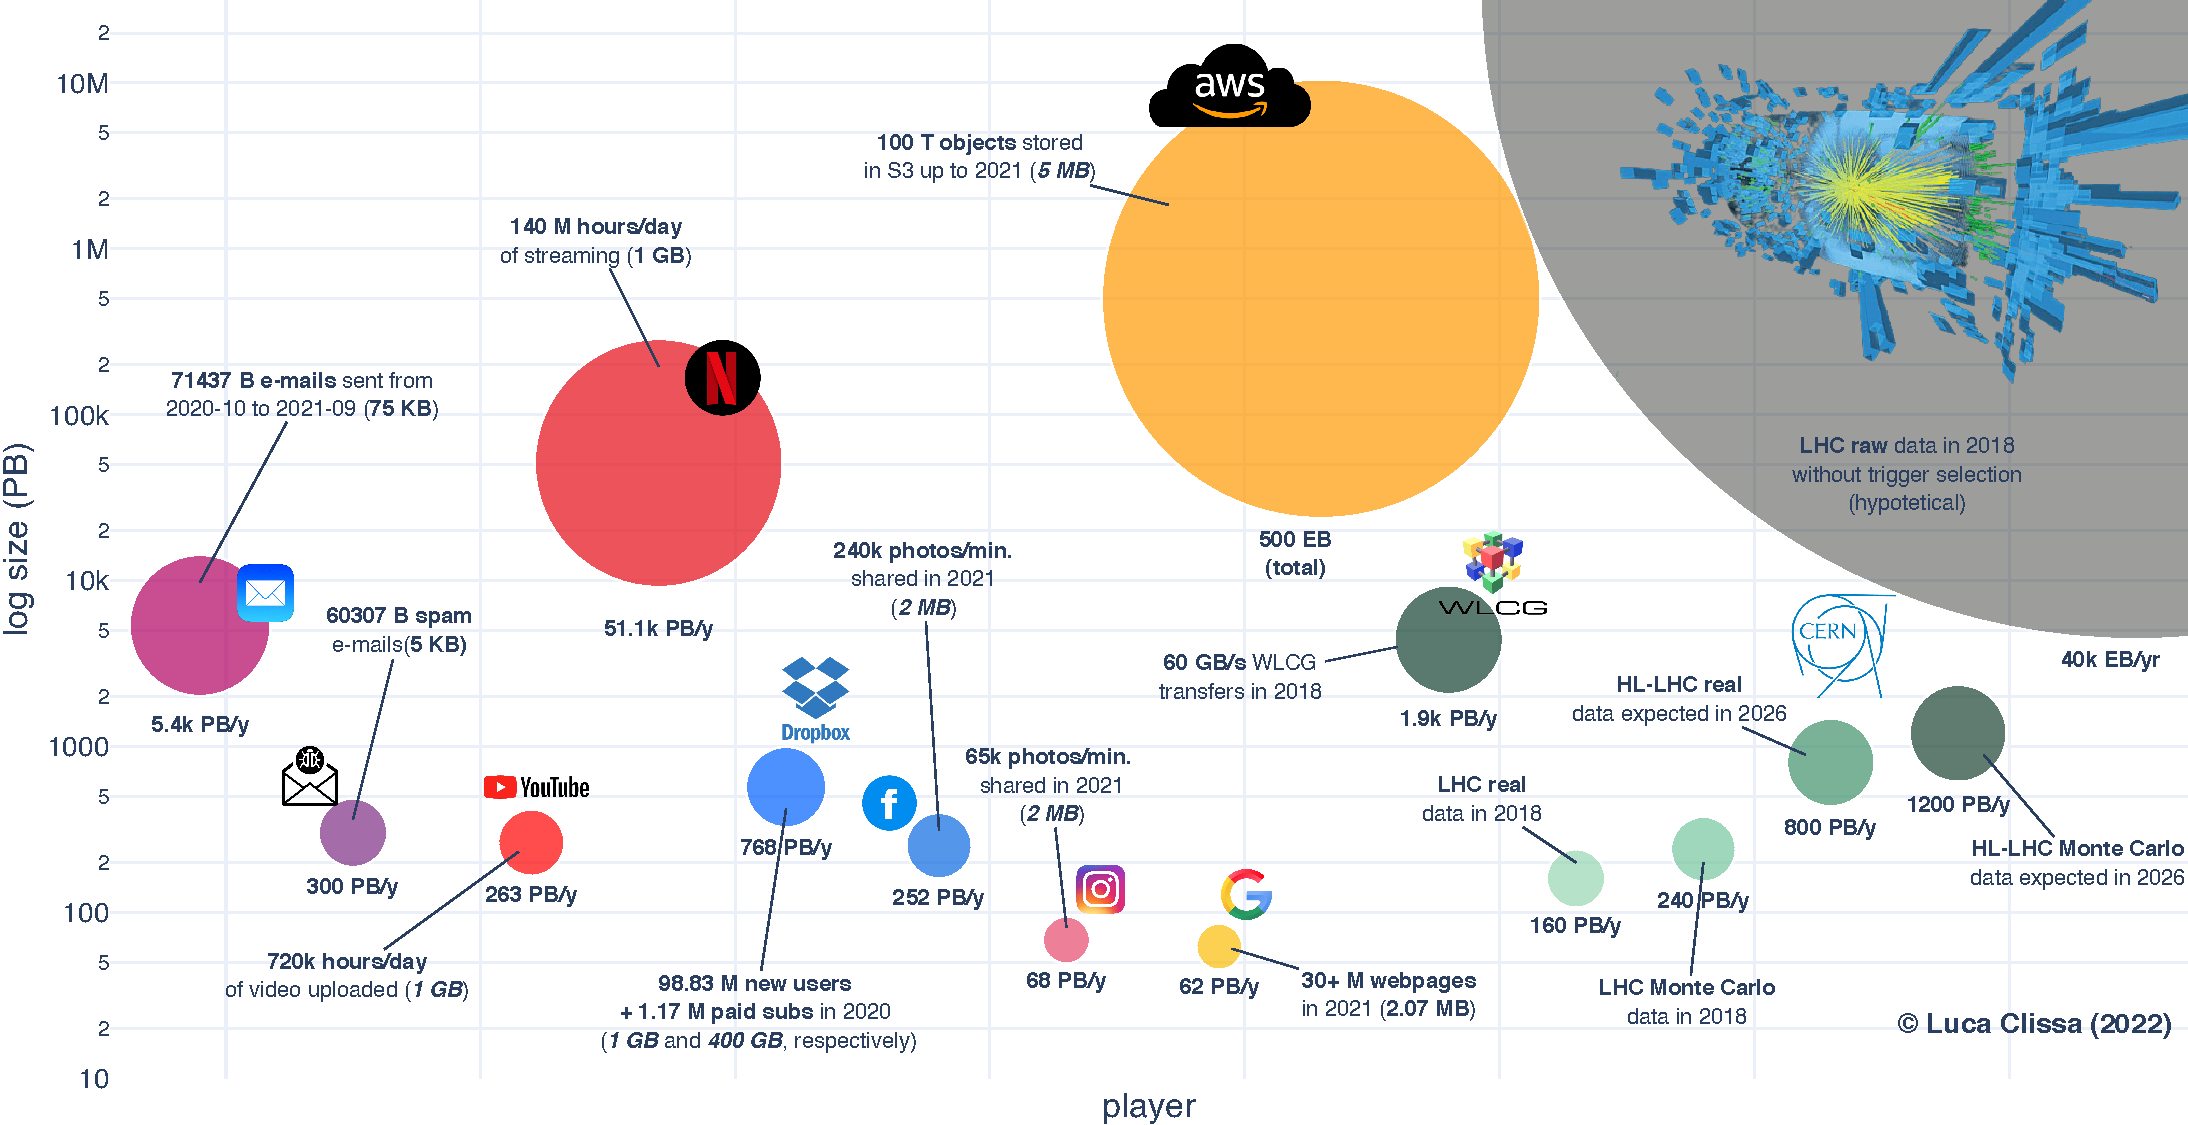
\includegraphics[width=\linewidth]{figures/220_introduction/BigData2021.pdf}};
% \begin{scope}[x={(image.south east)},y={(image.north west)}]
%     \node [anchor=west] (note1) at (0.26,0.170) {\href{https://stackoverflow.com}{Link}};
%         \node [anchor=west, scale=1, align=center,font=\tiny] (note2) at (0.26,0.470) {\href{https://rdcu.be/cB1Ds}{paper} \\ from the future};
% \end{scope}
%     \end{scope}
% \end{tikzpicture}
% \caption{\textbf{Big Data sizes.} Bubble plot of the orders of magnitude of data produced by important big data players. The balloon areas illustrate the amount of data and the text annotations highlight the key factors considered in the estimates. Average per-unit-sizes are reported in parentheses, where italic indicates measures reconstructed based on likely assumptions because no references were found.} \label{fig:bidata_size1}
% \end{figure}
% \end{landscape}
\begin{landscape}
\begin{figure}
    \centering
    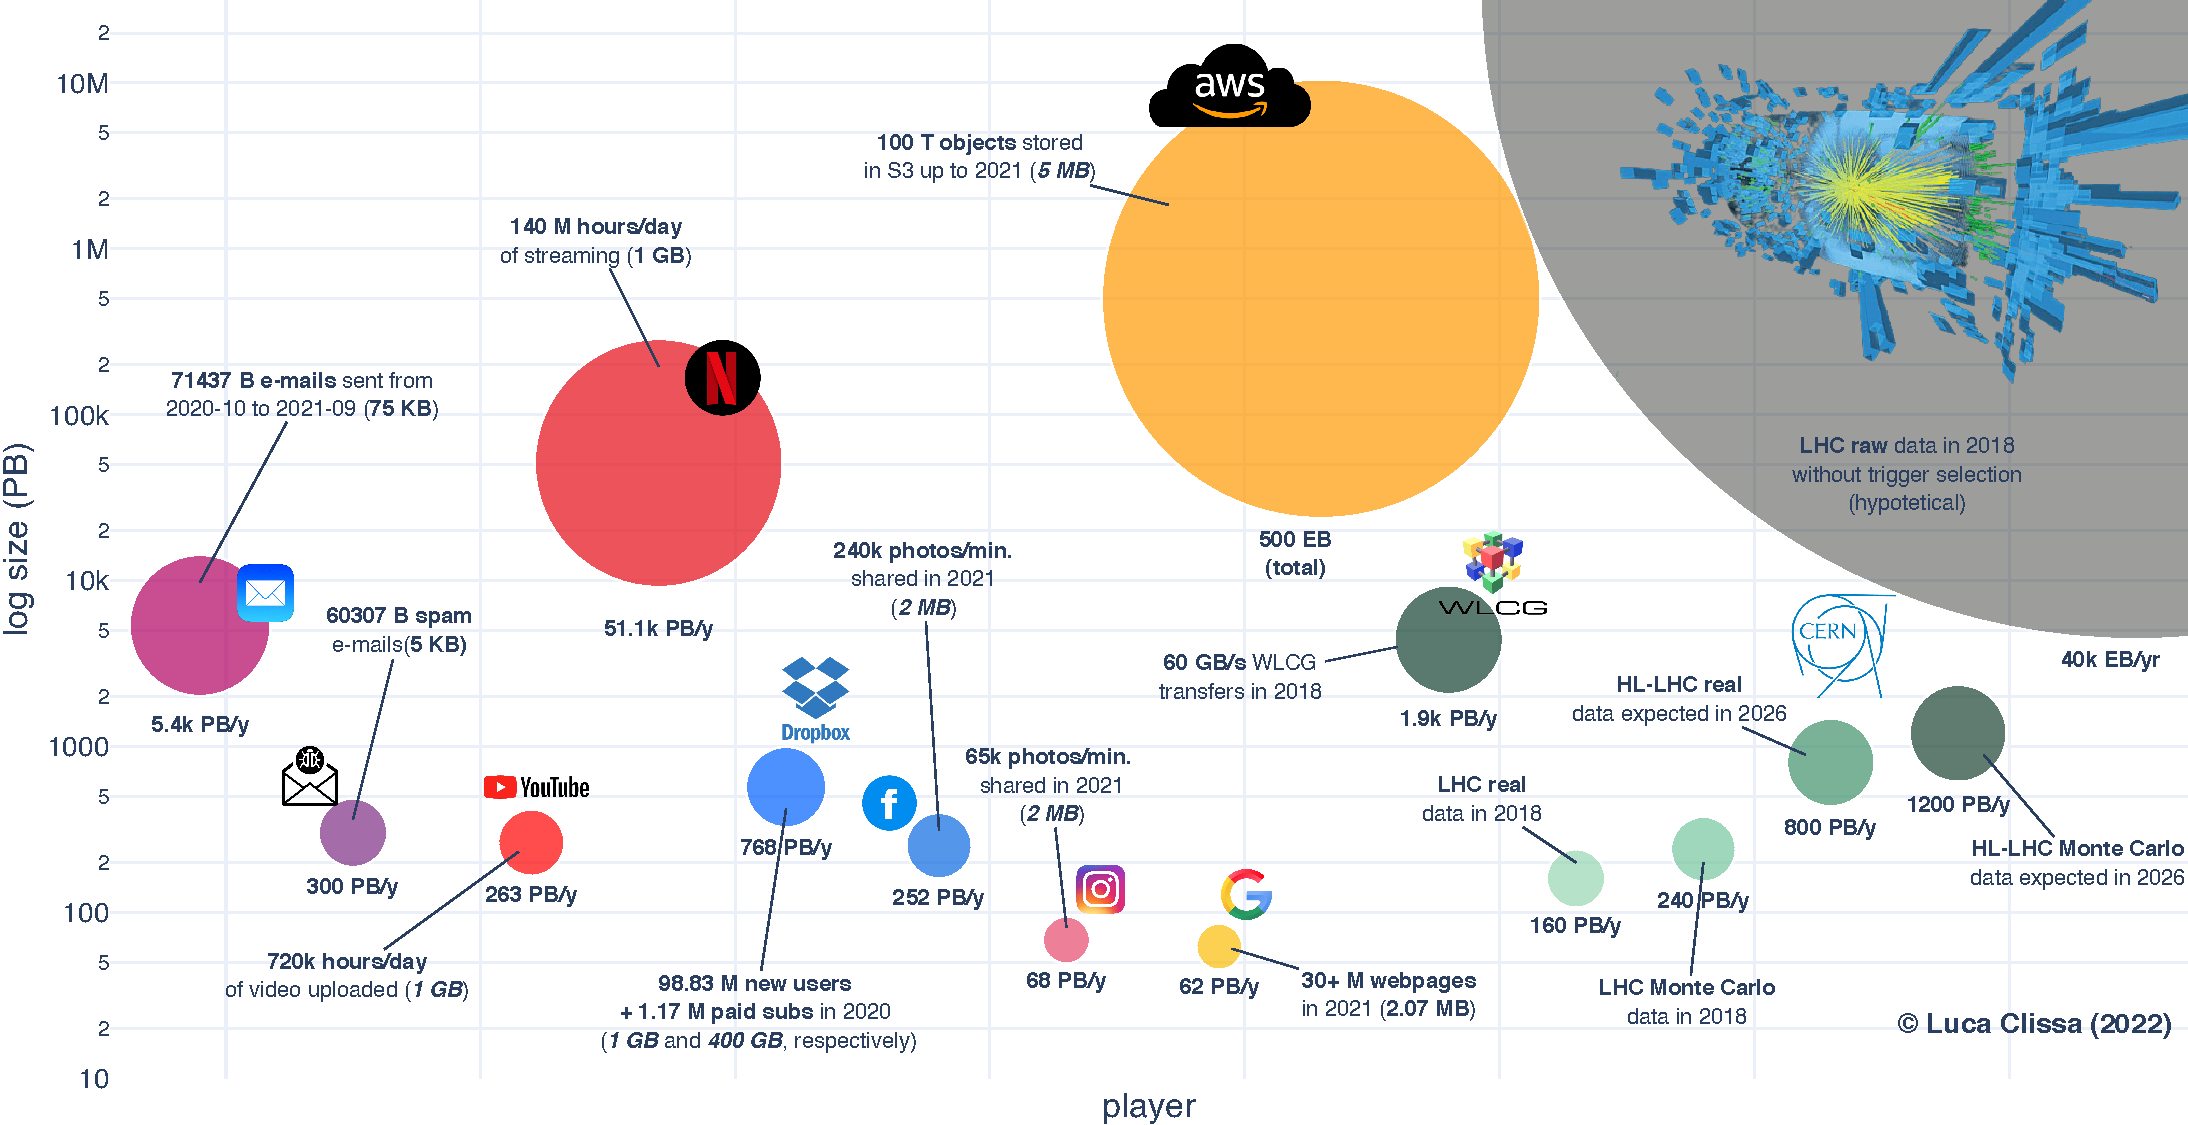
\includegraphics[width=\linewidth]{figures/220_introduction/BigData2021.pdf}
    \caption{\textbf{Big Data sizes.} Bubble plot of the orders of magnitude of data produced by important big data players. The balloon areas illustrate the amount of data and the text annotations highlight the key factors considered in the estimates. Average per-unit-sizes are reported in parentheses, where italic indicates measures reconstructed based on likely assumptions because no references were found. Interactive version available at: \href{https://clissa.github.io/BigData2021/BigData2021.html}{BigData2021.html}}
    \label{fig:bidata_size}
\end{figure}
\end{landscape}

Indeed the read-out data LHC produced every year in Phase 2 (40k EB) is around one order of magnitude bigger than the total size of objects ever stored on Amazon AWS cloud service (500 EB)%
\footnote{Obtained considering the total number of objects reportedly stored in Amazon S3 (100 trillion, \citeA{amazon2021objectscount}) and assuming an average size of 5 MB based on some average bucket example \cite{amazon2021objectssize}}.
Considering effectively recorded data, LHC figures are comparable with those of other most renowned big data entities. The last run (2018), in fact, produced hundreds of PetaBytes (PB) (roughly 160 of real data and 240 of Monte Carlo simulations),
 which is similar to the orders of magnitude generated by Google searches (62 PB)%
\footnote{Obtained considering that Google search index contains at least 30 billion webpages \cite{van2016estimating, google2021index_size, djuraskovic2020googl_stats, indig2020index_size} and that the average page size is 2.07 MB \cite{http2021webpage_size}
},
Instagram and Facebook shared photos (68 and 252 PB, respectively)%
\footnote{Obtained considering that 65k and 240k pictures are shared every minute on Instagram and Facebook \cite{domo2021infographic}, and assuming 2 MB as a reasonable average picture size \cite{adobe2021fb_img_size}
}
and YouTube video uploads (263 PB)%
\footnote{Obtained considering that 720k hours of video are uploaded daily \cite{domo2021infographic} and assuming an average size of 1 GB \cite{quora2021youtube}
}.
Moreover, LHC will climb the table even further with the upgrade to high luminosity, when the real and Monte Carlo data production rate is expected to rise to levels comparable to those of storage services like Dropbox (800, 1200 and 768 PB%
\footnote{Obtained considering that Dropbox registered 100 million of new users in 2020, of which 1.17 million were paid subscriptions \cite{dean2021dropbox}. For the average per-unit-size, it was assumed that free accounts exploited 75\% of the 2 GB storage available, while paid ones exploited 25\% of the total 2 TB
}, respectively). 

Apart from the nominal values of the generated information, streaming data comprise a significant slice of the big data market.
As a matter of fact, the continual movement of small- to medium-sized files spawns massive traffic when scaled up to millions of users, as testified by e-mails (5.7k PB)%
\footnote{Obtained considering that 71k billion e-mails and 60k billion spam messages were sent from October 2020 to September 2021 \cite{statista2021mails}, and that the average size is \mbox{75 KB} for e-mails \cite{lifewire2021avg_mail} and \mbox{5} KB for spam \cite{medium2014avg_spam}
},
and Netflix (51.1k PB)%
\footnote{Obtained considering that Netflix users consumed 140 million hours per day of streaming \cite{domo2021infographic} and that counts for 1 GB of data for standard definition videos \cite{perry2021netflix}
} bubbles in \cref{fig:bidata_size}.
% Also in this respect, LHC plays an important role. Indeed, the HEP community is formed by thousands of researchers spread around the world that need to access the data produced at CERN.
A similar usage is generated also by the LHC, whose data are continuously transferred across the HEP community thanks to the Worldwide LHC Computing Grid (see \cref{wlcg}) to fuel innovative research. For example, 
% 12 PB of data were accessed on average every day in 2020 for the ATLAS experiment alone \cite{calafiura2020design_report}, and
a throughput of 60 GB/s was generated by the 4 experiments together in 2018 \cite{wlcg2018throughput} thus giving a yearly projection (1.9k PB) close to half of the global e-mails traffic and only one order of magnitude lower than Netflix usage.
% Indeed, thousands of researchers from all around the world need to access LHC data, analyze them and share their results to investigate new theories and advance our knowledge of the universe.
% For this reason, the Worldwide LHC Computing Grid computing infrastructure has been developed over the years 

Given the large quantities of data involved by the LHC, it is not surprising how careful planning must be done in order to meet the needs of the LHC community, and tailored strategies and technologies must be adopted to cope with such requirements. 
Luckily, the presence of other stakeholders facing analogous problems provides the HEP community with some alternatives to draw from, and it allows researchers to tap in from existing solutions and customize them for their necessities.
    \section{The Worldwide LHC Computing Grid}
\label{wlcg}

The Worldwide LHC Computing Grid (WLCG) \cite{bird2011computing} is a global collaboration that links up more than 170 computing centers in 42 countries, serving an audience of more than 12000 physicists all around the world. 
As of 2022, WLCG constitutes the largest computing grid in the world and it is supported by many associated national and international grids, such as the European Grid Initiative and the Open Science Grid, as well as many other regional grids.
Founded in 2002 by CERN, the WLCG mission is to provide computing resources to store, distribute and analyze the data generated by the Large Hadron Collider.

Given the scale and complexity of the LHC data, this requires massive storage facilities, immense computing power, global networking, tailored software, adequate personpower and, of course, funding.
In order to achieve such challenging goals, WLCG leverages a distributed computing paradigm, where resources are shared among member states and made equally available to all the partners, regardless of their physical location.
% In brief, WLCG guarantees a seamless access to computing resources which include data storage capacity, processing power, sensors, and visualization tools, the resources that are capable to process over two million tasks daily, leveraging over one million computer cores and 1 exabyte of storage \cite{opint2022}.
\begin{figure}
    \centering
    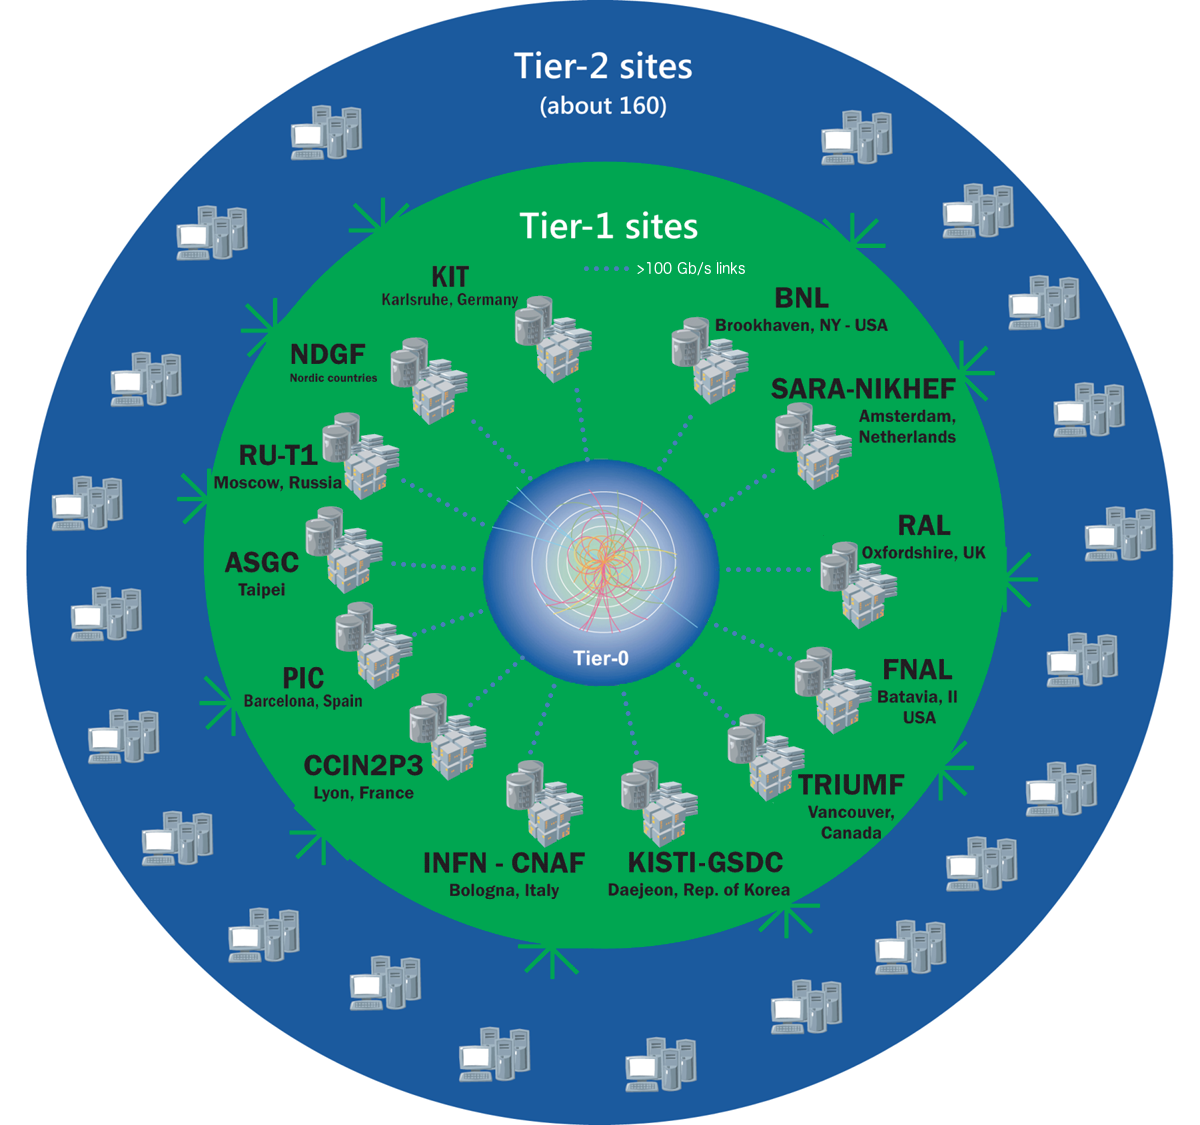
\includegraphics[width=\textwidth]{figures/220_introduction/WLCG-Tiers-2021_v3.png}
    \caption{\textbf{WLCG structure.} The Worldwide Large Hadron Collider Grid has a tiered structure organized into 4 levels and comprising more than 170 computing centers spread across 42 countries.
    } \label{fig:wlcg}
\end{figure}
\Cref{fig:wlcg} summarizes the WLCG infastructure composition. 
The Worldwide Large Hadron Collider Grid is structured in 4 levels, called \textit{tiers}, differing in terms of computing resources, storage capabilities and delivered services. 
% Proceeding from the bottom of this architecture, each layer sees an increased number
Its bottom layers comprise a few computing centers having great amounts of storage and processing resources, ultra-fast network connectivity (up to 100 GB/s), and they are devoted to general processing tasks.
The shallower layers, instead, group many smaller data centers devoted to more specialized activities.
In particular, the CERN data center is located at the bottom of this infrastructure, constituting the cornerstone of the whole architecture. 
It is located in Geneve (Switzerland) and it is endowed with more than 73000 processor cores, providing around 20\% of the total compute capacity of WLCG.
In terms of activity, the Tier-0 is responsible for i) the management of the raw data streams coming from the LHC experiments and their archiving for safe-keeping, ii) the reconstruction of physical entities like particles energy and velocity starting from the raw read-outs recorded by the electronic equipment, and iii) the distribution of raw and reconstructed data to the next tier layers.
Moving up the WLCG architecture, we find 13 large computer centres of the \textit{Tier-1s}.
These are directly linked to the Tier-0 and contribute to WLCG operations with sufficient storage capacity and round-the-clock support for the users. They are responsible for i) the safe-keeping of a proportional share of raw and reconstructed data, ii) large-scale reprocessing and safe-keeping of corresponding output, iii) access and distribution of data to the next infrastructure levels, and iv) safe-keeping of Monte Carlo simulated data.
One of these Tier-1 sites is located in Bologna\footnote{\cnaf} and it represents one of the biggest data centers in Italy. Its facilities count 40000 CPU cores, 40 PB of disk storage, 90 PB of tape storage, and the center is connected to the Italian (GARR) and European (GEANT) research network infrastructure with more than 200 Gbps \cite{cnaf2019annualrep, dell2019cnaf}.
The subsequent layer involves around 160 \textit{Tier-2} sites. These are data centers offered by universities and other scientific institutes, which are connected 
% to some of the Tier-1 sites 
through regional networks. 
They essentially act as analysis facilities to perform specialized tasks as the experiments production jobs and the Monte Carlo simulated data, which are then either stored locally or shared across the infrastructure.
% Despite having storage resources, the Tier-2s are not required to archive data, so the outputs produced there are typically sent back to Tier-1s when they are intended to be shared (as in the case of Monte Carlo data).
Finally, the last rung of the ladder is constituted by \textit{Tier-3s}. These sites enormously vary in scale,  ranging from local computing resources like university clusters or even individual pc to large national analysis facilities.
In fact, they do not formally belong to the WLCG but solely serve as entry points to its infrastructure for end-users analyses.

Alongside the hardware facilities, the WLCG supplies also advanced software solutions to provide researchers with seamless access to resources in a transparent way, without needing to worry about where the computing resources are coming from or where the data are physically stored.
This means that users can request access to data or resources from one of the many entry points into the system, and the grid infrastructure will then take care of spawning all the needed processes under the hood.
This may entail establishing the user identity and its access rights to the various sources, checking their credentials, and searching for available sites that can provide the requested resources.

\chapter{Infrastructure management} \label{ch:opint}
The automation of infrastructure management and maintenance has become crucial in recent years. 
The increasingly large scale of modern data centers, and the adoption of distributed resources that necessitate the interaction of diverse hardware and software components, have made this task extremely complex. Consequently, traditional approaches to infrastructure management where manual human intervention is required have become impractical or even useless. 
For this reason, several strategies were proposed to support operational workflows in various ways \cite{opint2020, opint2022, decker2020powerquality, diotalevi2019elk}.
Although listing a precise taxonomy of alternative methods is hard -- since the boundaries between different classes are often blurred and the categories may overlap -- a first distinction can be established based on the analysis intent.
A common approach is to focus on \textit{anomaly detection}, where the objective is to spot anomalous behaviors that may entangle underpinning faults in the system. The detected anomalies are then reported to experienced operators for further investigations and fixes.
However, sometimes the malfunctions are too many to be inspected and solved singularly. Hence, an option is to rely on \textit{error categorization} to reduce the number of reports to check by grouping similar issues. This approach assumes that similar problems have similar solutions, therefore it is possible to address all the events of a group by inspecting only one (or a few) of them.
A more desirable yet more complicated target is \textit{root-cause analysis} \cite{sole2017survey}. In this case, the objective is to identify the origin of the problem directly, thus entirely automating the diagnosis phase.
In turn, these approaches can be further split into methods that seek just root causes -- what induced the issues -- or plain explanations -- why/how the faults were conceived.

Another essential distinction is based on the time of intervention with respect to a system failure. 
The simplest approach is \textit{reactive maintenance}, where the human intervention occurs after a failure is detected. In this case, the fault diagnosis is performed \textit{post-mortem} and, if effective, it helps identify the problems and speed up the restoration of good operating status. 
Nonetheless, the failures are not avoided and downtimes or denial of services are impossible to avert.
Some approaches try to intervene proactively to overcome this limitation, performing the so-called \textit{preventive maintenance}. In this case, the objective is to set an optimal schedule of periodic interventions to preserve high Quality of Service (QoS) and prevent faults directly.
However, completely eradicating failures requires frequent maintenance that is often unnecessary, which increases management costs.
An alternative strategy to limit these extra expenses is \textit{predictive maintenance}. The idea is to monitor the infrastructure on the fly (\textit{real-time} or \textit{online} analysis) and try to predict when an intervention is required. In this way, the inconveniences deriving from system downtimes are limited, and the costs imputable to unnecessary hardware replacement are cut.

Apart from the end goal and the time requirements of a given use case, a further distinction can be established based on the analyzed information.
Indeed, the choice of which strategy to pursue is bound by the available data or, vice-versa, it restricts the applicable techniques.
A first family of approaches leverages overall workloads -- e.g. number of running processes, hardware resources usage, network saturation -- as indicators of infrastructure health and monitor their trends over time. The deviations from normal operations are considered anomalies and trigger alerts to be investigated by experts \cite{paltenghi2021}.
A second class relies on \textit{event logs} as the primary way to register key runtime information. These reports record events happening during the execution of a system to provide an audit trail that can be helpful to understand the system activity and diagnose problems.
This information can be exploited in various forms.  
Some approaches focus on log activity summary statistics (e.g. number of printed lines) and try to disentangle nominal behaviors from suspect activity \cite{decker2020fuzzy, decker2020granular, minarini2020time}. 
Other alternatives use the log content instead, thus directly analyzing the textual information contained in the log files \cite{giommi2019predmaintenance}. These vary from traditional keyword searches -- e.g. ``kill", ``error", ``fail", ``exception" -- and heuristics \cite{tisbeni2019} to smarter tools based on deep learning language models.
The advantage of such procedures is that the textual information can aid system experts finding root causes and explanations which are harder to grasp from sheer workloads.
Both families mentioned above can be adopted for both online monitoring and offline debugging, depending on the use case.
Finally, another class of techniques focuses on \textbf{error messages} and is only devoted to diagnosing issues in post-mortem analyses. Like event logs, errors can be exploited to conduct thorough root-cause investigations or just error categorization.
Although logs and error messages both collect textual data, their difference lies in the format this information is presented in and the actual content. 
Error messages only include system printouts related to failure events, while logs typically gather the full runtime information. 
In terms of format, error messages are cleaner compared to log files, despite both can be listed as semi-structured data. 
In fact, both classes can be summarized into a free-form constant string describing the status of a system, plus some parameters that record important system attributes.

This work tackles the problem of error categorization for post-mortem diagnosis of issues during WLCG data transfers.


    \section{Distributed data management}
\label{ddm}

LHC data are arguably the most valuable asset of the HEP community.
As a consequence, the data are continuously transferred across the grid for several purposes, and a paramount part of the WLCG operations involves Distributed Data Management (DDM) processes.

Indeed, stringent workflows are put in place by the experiments to ensure data distribution and redundancy, thus preventing data loss and guaranteeing reliable accessibility.
For example, the ATLAS experiment has drawn up an accurate plan -- the so-called \textit{computing model} -- describing in detail the data life cycle \cite{aad2008atlas, calafiura2020design_report, bird2011computing}.
The first data stream happens at the CERN data center, where a combination of electronic and software triggers are applied to the raw data acquired by the detectors to filter out uninteresting collisions.
The skimmed data are then archived in the Tier-0 on tape supports for long-term storage, and a second copy is sent to one of the Tier-1s through a dedicated network. 
After that, a first-pass reconstruction occurs to retrieve physically meaningful information -- such as particles energy, velocity, scattering angles and so on \sidenote[Luca][notesyellow]{sono giuste queste grandezze?} -- from the electronic signals recorded by the experimental devices.
As for the raw data, these elaborations are stored in double copy, one at CERN and one at the same Tier-1 hosting the corresponding raw data.
In this way, two full copies of the same raw and reconstructed data are retained to safeguard data accessibility and recovery.
The copy at CERN is archived on durable but slow storage supports, and it serves the purpose of restoring the data in case of losses or corruption. The second copy, instead, is stored on hard drives that are more prone to faults but guarantee a faster reading speed to comply with the repeated data accesses typical of analysis workflows.
Once the data are properly distributed, a second stream takes place at the Tier-1s that provide data-intensive processing facilities for large-scale organized analysis. Here, further (re)processing and calibrations are performed on the reconstructed data, and the derived outputs are stored and shipped on-demand to other sites for subsequent elaborations.
The last part of the data life cycle is then performed at the Tier-2s, where Monte Carlo data are simulated and sent back to Tier-1s for long-term storage. 
Furthermore, the Tier-2s are exploited by smaller groups of researchers to conduct more specialized analyses. In such cases, additional data streams are needed to retrieve the reconstructed data from the Tier-1s and make the results available to the end-users on their local machines.

% On the other hand, analysis workflows require individual researchers to transfer data of interest for their analyses.
% This potentially requires retrieving data from geographically displaced and heterogeneous storage resources (e.g. tape or disk), transferring them to computing resources that may be situated elsewhere, and transferring the results back to their machines in order to conduct their studies.
    \section{FTS transfer failures} \label{sec:FTS_failures}


In practice, occasional faults may happen at various levels during data transfers, which may include a wide range of root causes, provoking failures during the shipment of the files.
These errors may vary from naive ones -- e.g. a mistyped command or the request of an unavailable file -- to more severe software and hardware defects.
For instance, the requesting endpoint or archiving server might be temporarily unreachable (connection shortage).
Likewise, the requested data may be corrupted (checksum error) due to storage hardware faults or unstable connection (network problem).
Also, there might be timeouts when the shipment takes more than the pre-configured waiting window -- e.g. when the desired data are bigger than usual and/or must be retrieved from tape, thus requiring more time.
In addition, errors of different nature may often arise due to the interactions between miscellaneous middleware layers.
All of these factors, and more, can generate significant service disruptions and infrastructure malfunctions that require prompt intervention.
For this reason, data transfer processes are continuously monitored by teams of shifters. When an issue is detected, the operators report it through the Global Grid User Support (GGUS) ticketing system \cite{antoni2008ggus}, and experts and site maintainers take care of their solution.
To give an idea of the volumes involved, the ATLAS collaboration alone experienced an average traffic of more than 2 PB per day in 2019 \cite{calafiura2020design_report}, corresponding to roughly 1.5-2 million files moved each day.
Nearly 10\% of these transfers failed producing about 100-200k errors on a daily basis. 
In total, transfer failures generated more than 4k incident reports filed in 2019\footnote{\ggus} for all the LHC experiments (1141 for ATLAS only).
Due to the complexity of the infrastructure and its layered composition, understanding the problem root causes and fixing them demands a great human effort -- more than 100 ATLAS members were involved in 2019, corresponding to roughly 50 FTEs (Full-Time Equivalent)~\cite{jarka2019ftes} -- and it may entail undesired disservices.
The average solving time, may vary from a few hours or days -- e.g. in the case of issues that are easy to solve or have already been dealt with in the past -- to entire weeks -- e.g. for unknown problems or more troublesome malfunctions that imply important software or hardware interventions.
In practice, the median solving time for incidents reported by the ATLAS, CMS and LHCb collaborations in 2019 was around 17 days, with a 90\textit{-th} percentile of 44 days and a long right tail extending over 100 days (see \cref{fig:ggus_time}).
\begin{figure}
    \centering
    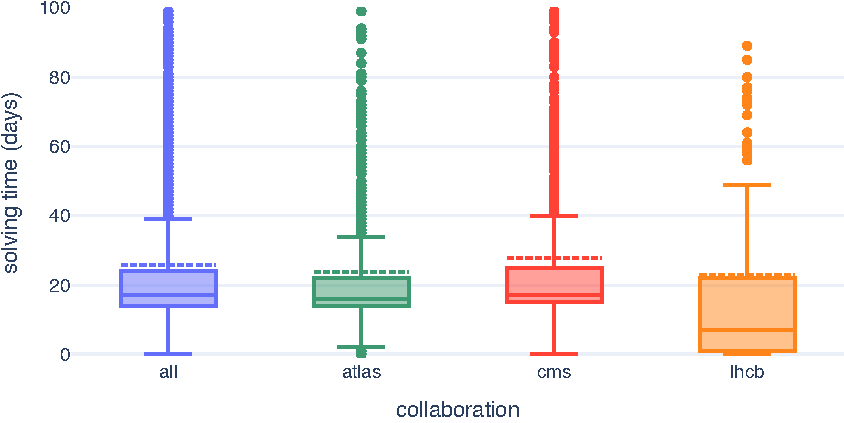
\includegraphics[width=\textwidth]{figures/220_introduction/GGUS_time.pdf}
    \caption{\textbf{Tickets solving time.} Boxplot of the distribution of the solving time for GGUS incidents reported in 2019 by ATLAS, CMS and LHCb collaborations.}
    \label{fig:ggus_time}
\end{figure}
When a transfer failure happens,
the FTS log files are parsed and the transfers more relevant features are extracted and re-organized in a structured format. 
In particular, this involves collecting the exit status of each of the subsystems responsible for the transfer and appending them to compose a global error message.
This information is then exposed to the on-duty shifters along with other characteristics -- e.g. source and destination endpoints, file size, exchange protocol and so on -- and visualizations -- e.g. time evolution plots or site transfer efficiency -- for more in-depth investigations.
% \lc{Here goes some reference to the orders of magnitude at stake, i.e.: 
% \begin{itemize}
%     \item n. tranfers/day (whole or per virtual organization) --> can retrieve from FTS
%     \item ticket/year or month or day (whole or per virtual organization) --> how to retrieve that? is there any official source?
% \end{itemize}
% }

% \lc{Describe current operations and possibly volumes: 
% \begin{itemize}
%     \item Current operations: efficiency matrix + drill down (description + falls)
%     \item average solving time $\rightarrow$ how to retrieve that? is there any official source?
%     \item n. people involved (both shifters and sites) $\rightarrow$ how to retrieve that? is there any official source?
% \end{itemize}
% }
%Current operations are based on a site-centric monitoring approach that involves mainly manual, post-mortem reporting. In this approach, trained operators look at Grafana dashboards that act as a high-level overview of the systems status and try to spot hints of incorrect or undesired behaviours.
Current operations are based on a \textit{site-centric} approach where trained personnel monitors the status of the various services almost 24/7 and tries to spot hints of incorrect or undesired behaviors. In particular, the operators look at Grafana dashboards to get a high-level overview of the system. A usual starting point is the so-called efficiency matrix (\cref{fig:efficiency_matrix}), where the percentage of successful transfers is reported. The granularity level is customizable and it may range from global transfers between national cloud infrastructures involving more computing centers to a finer tracking of particular site exchanges or even specific endpoint links. 
When the efficiency falls below an acceptable threshold, typically 60-70\%, on-duty shifters start to investigate the issue at a lower level by checking \emph{i)} where the error happened, \emph{ii)} how many errors are produced, \emph{iii)} what is the time pattern (temporary, extended or cyclical) and \emph{iv)} which error messages are generated. 
However, this procedure gives rise to many false alarms as it is usual to encounter problems that do not represent a real concern. For instance, this may happen when few transfers are attempted so even a low number of errors imply a high failure rate, or when there are after-effects of a transient issue that had already been fixed. 
Also, sometimes unnecessary drill-down activity is performed for actual issues that were already known, as in the case of ongoing tickets or site downtimes, for which reporting is not required.
As a result, many human resources are employed in repetitive tasks of little scientific interest that would enormously benefit from automation. 

In addition to that, the site-centric strategy described above has some drawbacks. Firstly, monitoring focuses on spotting where issues occur, while understanding the actual root causes is typically demanded to site experts in a subsequent investigation.
Secondly, problems generating few error messages are usually ignored. This is natural, and to some extent desirable, as having limited resources forces us to address bigger malfunctioning first. However, that could be a potential pitfall in cases where promptly fixing a minor issue may prevent the rising of a more significant and longer to solve defect.

All these problems could be tackled programmatically by standardizing the logging output of all the services. In this way, neat error messages would point directly to the source of the problem, thus allowing complete automation. 
However, the distributed nature of the infrastructure hampers such an approach.
In fact, the opportunistic gathering of computing resources that led to WLCG entails many local configurations that are not easy to address using only a static strategy.
Therefore, all these considerations expose the need for an intelligent support tool for speeding up infrastructure management to meet the productivity requirements for the near future.

\begin{landscape}
\begin{figure}
    \centering
    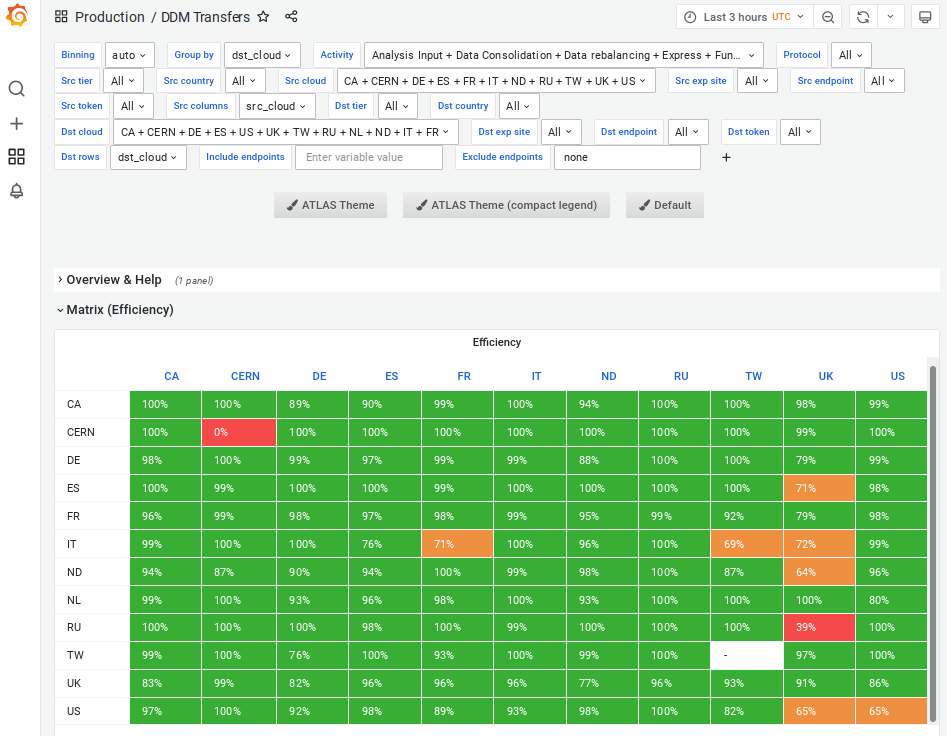
\includegraphics[height=\textwidth]{figures/220_introduction/grafana_efficiency_matrix_narrow1.png}
    \caption{\textbf{Transfer efficiency matrix (Grafana)}. Transfer sources are shown as columns and destinations as rows. The drop-down menus at the top allow for custom filtering at the desired level of granularity.}
    \label{fig:efficiency_matrix}
\end{figure}
\end{landscape}
    \subsection{Related works} \label{sec:related_opint}


Analyzing error messages encountered in large-scale distributed systems has become one of the crucial tasks for monitoring computing resources. 
Thus, a variety of tools for log and error message parsing has already been explored. 
Some of these approaches include longest common subsequence \cite{du2016spell}, frequent pattern mining \cite{vaarandi2003slct, vaarandi2015logcluster}, iterative partitioning \cite{makanju2009iplom}, parsing trees \cite{he2017drain} and  hierarchical clustering \cite{fu2009lke} (see \citeNP{zhu2019tools} for a thorough discussion and comparison).
However, the existing tools present some drawbacks. First, most methods require a crucial pre-processing phase that may need deep customization for specific data. This limitation hampers their adaptation to novel use cases as different systems may have diverse logging conventions, terminology and structure.
Furthermore, they do not allow error messages to be linked with additional entities other than the textual information, meaning that messages cannot be clustered along with auxiliary data.

% These approaches are typically made of two stages: \textit{i)} text vectorization and \textit{ii)} clustering.
% The first step is needed to transform the textual information into a convenient numeric representation.
% Once that is achieved, the resulting data are grouped thanks to clustering algorithms of various kinds. 

\citeA{clusterlog2021} presents a pipeline consisting of several stages specifically tailored for data processing workflows within WLCG. 
First, the error messages are tokenized\footnote{\label{note1}for more details see \cref{sec:vectorization}} and cleaned from digits, punctuation and special characters.
Then, a hashing algorithm replaces the parametric parts of the message with a placeholder, and the resulting patterns are exploited for the following elaborations. In this way, the total amount of data is reduced by 90-95\%.
After the above pre-processing, the vectorization\footnoteref{note1} stage is based on \textit{word2vec} \cite{mikolov2013word2vec} that computes a numerical representation for each token. The overall message representation is then retrieved by averaging over single word embeddings.
% (see \cref{sec:vectorization} for more details). 
The resulting representation is then reduced in dimension by means of principal components analysis \cite{wold1987pca}, and a DBSCAN \cite{ester1996dbscan} algorithm is adopted for the clustering stage.
Finally, cluster descriptions are extracted by searching common textual patterns and key phrases for all messages belonging to the same cluster.
% Although this pipeline accounts for most needs of typical workflows concerning error messages, it also presents some drawbacks.
% First, the pre-processing and vectorization stages reduce all the principal sources of variability, turning the whole approach into something close to unique strings grouping (assuming a smart and flexible definition of unique strings). 
% For example,  the raw error messages are transformed into structured templates where the same placeholder replaces parametric parts.
% This choice drastically decreases the data variability. Also, it hampers the usage of parameter values for error discrimination, potentially masking faults due to specific components, e.g. one particular file is corrupted and needs restoration, or a determined site/service is not responding.
% Moreover, performing principal components decomposition on the word2vec embedding further reduces the expressive power of the learned representation.
% Although the previous strategies are crucial to comply with the runtime and computing requirements of particular use cases, they seem to contrast the current best practice for text processing. 
% In fact,  the recent applications in NLP literature suggest exploiting the increased computing power of modern architectures to train bigger models with minimal hard-coded pre-processing. 
% The idea behind that is to let the model figure out linguistic features -- e.g. grammar, syntax, lexicon, semantic -- and relations among tokens, thus endowing the resulting model with increased expressive power.
% As a result, the previous strategies likely hinder learning an optimal embedding, perhaps questioning the need for the word2vec language model for text vectorization in the first place.
% As a second drawback, no auxiliary information concerning the precesses is considered alongside the error message. 


Another interesting approach is presented in \citeA{lin2016log}, where the authors propose a convenient pipeline to group logs of failed jobs and exploit the knowledge coming from previous failures.
After substituting placeholders instead of parametric parts in the raw messages, each log is summarized using the unordered set of the events (log lines) it contains.
A vectorization stage is then performed based on Inverse-Document event Frequency (IDF) and contrast-based weighting. 
The resulting numerical representation undergoes an agglomerative hierarchical clustering algorithm that finds groups of similar logs.
The resulting cluster centroids are then taken as representative log sequences of their respective groups, and they are compared to a knowledge base of previous failures and corresponding solutions. If the sequence similarity to one of the known issues is above a given threshold, the corresponding actions are applied to solve the problem. Otherwise, the log sequence is passed to system experts for manual inspection and the reference dataset is successively updated.
In this way, human resources are involved only in handling new issues, while previous knowledge is exploited for recurrent ones.

Another way to look at this problem is through the lenses of Natural Language Processing (NLP), where related tasks have been addressed by adopting various strategies.
A direct approach would be to regard error categorization as a specific example of topic modeling \cite{hofmann1999probabilistic, papadimitriou2000latent}.
In brief, topic modeling resorts to a low-dimensional latent representation of textual data where each latent dimension may be interpreted as a separate topic.
In the context of error categorization, the different topics can be seen as high-level descriptions of different failures, and the messages as particular instances of the related problems.
Alternatively, popular \textit{language models} can also be leveraged \cite{devlin2018bert, peters2018elmo, brown2020gpt3}.
They consist of numeric representations for textual information -- also known as \textit{embeddings} -- that preserve syntactic, grammatical and semantic relations of the original data, but in a lower dimension. 
This means that words similar in terms of meaning and usage are projected near to each other.
Therefore, these techniques can be adopted to get convenient error embeddings where related failures are close in the sense of some distance or similarity measure, and clustering algorithms can be exploited to retrieve error categories.


    \section{Contribution}
The goal of this work is to discuss a complementary approach to current operations based on an experiment-agnostic, computer-aided strategy to grid monitoring centered on error messages rather than site performances.
In particular, we propose an unsupervised Machine Learning (ML) pipeline to identify clusters of similar failures. The groups of errors retrieved in this way are then exposed to shifters as suggestions of potential issues to investigate further.


\chapter{FTS transfer failure analysis} \label{sec:pipeline}

The general idea is to start from a collection of textual data, corpus, formed by documents of various lengths and scope.
The available information is then analyzed to retrieve groups of documents sharing similar content, and the matching patterns are interpreted as topic descriptions.
Of course, the string format of the raw data is highly unstructured and impractical to handle, thus limiting the plethora of applicable techniques. 
For this reason, the (possibly long) strings incorporated in the documents are first quantized into unitary pieces of textual information, tokens, from which the raw strings can be reconstructed. These process may vary from simply using words \cite{bengio2003word, mccann2017word} or characters \cite{ling2015char, dhingra2016char}, to more complex strategies involving subwords \cite{gage1994subword, sennrich2016subword}, sentences \cite{kiros2015sentence}, documents \cite{le2014documents} and topics \cite{niu2015topic}. 



Our work is inspired by the approach described in \cite{lin2016log}, although only part of the pipeline has been developed since no knowledge base is available for our use case.
Also, our work is conceptually similar to the work of \cite{clusterlog2021}, although some major differences are present in the pre-processing, clustering and description stages.

\sidenote[Luca][notesyellow]{Confronto con pipeline di Maria e argomentazione differenze}
Although this pipeline accounts for most needs of typical workflows concerning error messages, it also presents some drawbacks.
First, the pre-processing and vectorization stages reduce all the principal sources of variability, turning the whole approach into something close to unique strings grouping (assuming a smart and flexible definition of unique strings). 
For example,  the raw error messages are transformed into structured templates where the same placeholder replaces parametric parts.
This choice drastically decreases the data variability. Also, it hampers the usage of parameter values for error discrimination, potentially masking faults due to specific components, e.g. one particular file is corrupted and needs restoration, or a determined site/service is not responding.
Moreover, performing principal components decomposition on the word2vec embedding further reduces the expressive power of the learned representation.
Although the previous strategies are crucial to comply with the runtime and computing requirements of particular use cases, they seem to contrast the current best practice for text processing. 
In fact,  the recent applications of Natural Language Processing (NLP) suggest exploiting the increased computing power of modern architectures to train bigger models with minimal hard-coded pre-processing. 
The idea behind that is to let the model figure out linguistic features -- e.g. grammar, syntax, lexicon, semantic -- relations among tokens, thus endowing the resulting model with increased expressive power.
As a result, the previous strategies likely hinder learning an optimal embedding, perhaps questioning the need for the word2vec language model for text vectorization in the first place.
As a second drawback, no auxiliary information concerning the precesses is considered alongside the error message. 

One of the main concerns in data transfer operations is to promptly detect and solve issues that affect the functioning of the infrastructure.
On our way towards improving automation of DDM operations, we adopted an unsupervised learning approach to minimise experts' effort and enable discovering new failure patterns related to FTS transfers. 
The pipeline consists of 
% can be summarised into 
two main steps: \textit{i)} vectorization and \textit{ii)} clustering.
In the {\emph{vectorization step}} we concatenate the raw error string with source and destination hostnames and we use a word2vec model that learns how to map all that information to a vectorial space of a given size, where similar errors are expected to be close together. This is to transform the textual information into a convenient numeric representation and serves as preprocessing for the next steps. 
A {\emph{clustering algorithm}} is then applied to group related errors: 
% In practice, the idea is to 
we pre-train a word2vec model on a big dataset 
-- possibly updating it once in a while -- and then 
and run a \mbox{K-Means++} algorithm \cite{kmeans} online during the monitoring shifts.  
% 

In order to demonstrate the approach, we report an analysis of FTS data from one full day of operation. %(15/01/2021).
\cref{fig:cluster0} shows an example of a summary table for the biggest cluster found by the model.
\begin{figure}[t]
    \centering
    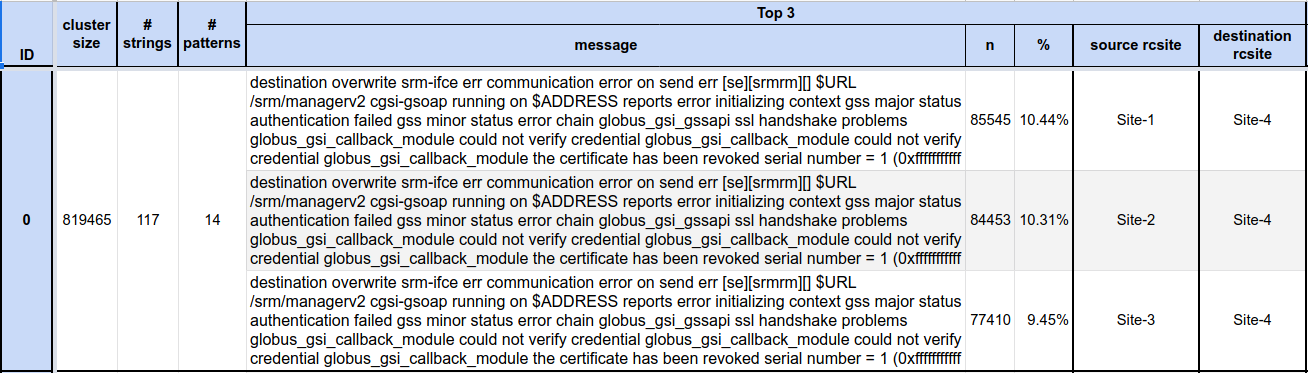
\includegraphics[width=\textwidth]{figures/410_method/cluster0_wide.png}
    \caption{
    % Example of cluster summary for cluster 0, the biggest cluster found by the chosen model. % 
    Example of an error message cluster summary.}
    \label{fig:cluster0}
\end{figure}
The first three columns provide numeric summaries: \textit{i)} the cluster size, \textit{ii)} the number of unique strings within the cluster, and \textit{iii)} the number of unique patterns: unique strings after the removal of parametric parts like paths, IP addresses, URLs and so on. The model learns to \textit{abstract} message parameters and to group strings that are similar except for the parametric parts. As a result, the initial amount of errors is reduced to a number of patterns which is lower by several orders of magnitude. 
The core part of this visualization is then represented by the \textit{Top 3} section, where the most frequent triplets of pattern, source and destination sites are reported in descending order, together with their multiplicity and the percentage over the cluster size.
There we extract several insights, for example whether a pattern is responsible for a large number of failures or if it accounts for a conspicuous fraction of the cluster. In addition, one can investigate the contribution of source/destination site pairs, 
% Also, one could look at whether errors are concentrated in a specific source/destination site, 
as in \cref{fig:cluster0} where Site-4 clearly seems to have a problem as destination. 
%
Another useful piece of information is given by the cluster's time evolution plot (shown in \cref{fig:timeplot_cluster0}) that can give an immediate indication of whether the problem  is transient or not. 

% \begin{wrapfigure}{hR}{0.53\textwidth}
\begin{figure}
    \centering
    % \vspace{-8mm}
    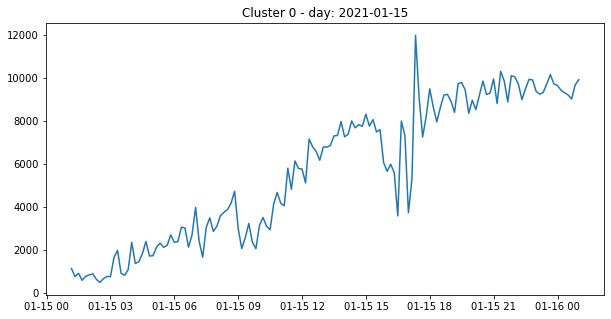
\includegraphics[width=\textwidth]{figures/410_method/timeplot_cluster0.png}
    \caption{Time evolution of cluster 0: the plot shows the count of errors in bins of 10 minutes.\vspace{3mm}\phantom{.}}
    \label{fig:timeplot_cluster0}
    % \vspace{-10mm}
\end{figure}
% \end{wrapfigure}

%
Overall, the idea is for the shifters to look at summary tables and time plots for each of the clusters detected by the algorithm, which act as suggestions of possible issues to investigate further, or later, would create automatic alerts, notifications, or even issue reports. 

\newcommand{\specialcell}[2][c]{\begin{tabular}[#1]{@{}c@{}}#2\end{tabular}}
\begin{table}[htb]
\centering
% \resizebox{\textwidth}{!}{
\begin{tabular}{cccccccc}
\toprule
\textbf{N. Clusters} &  \textbf{ASW} &  \textbf{WSSE} &  \textbf{\specialcell{Perfect\\Match}} &  \textbf{\specialcell{Fuzzy\\Match}} &  \textbf{\specialcell{Partial\\Match}} & \textbf{\specialcell{False \\ Positives}} & \textbf{\specialcell{False \\Negatives}} \\
\toprule
     &       &        &     &    &    &    &   \\[-0.25cm]
  15 &  0.89 &  17107 &   7 &  3 &  2 &  3 &  1 \\[0.2cm]
\bottomrule  
\end{tabular}
% }
\caption{Summary of pre-validation results.}
\label{tab:crosscheck}
\end{table}

The process described above can be fully automated after tuning model hyper parameters based on metrics such as Average Silhouette Width score
% (ASW)
and Within-cluster Sum of Squared (Euclidean) distances, that measure how compact and separated the clusters are.
However, this is not directly related to the meaning of the messages being grouped. Hence, this is to be intended as a proxy of a correct model behaviour rather than a real performance metric.
For this reason, 
We have conducted an extensive testing as pre-validation comparing the clusters obtained with this approach against GGUS tickets, showing a reasonable overlap between suggested and reported issues. 
In particular, for the analysis above we considered issues reported in a skewed time window of 17 days (1st to 18th January) so to include both known issues and the ones possibly spotted with some delay.
Results of this cross-check are reported in Table \ref{tab:crosscheck}.

The model found 15 clusters reaching ASW and WSSE of 0.89 and 17107, respectively. The results show a good agreement, with 7 perfect matches (both reported message and affected site), 3 fuzzy matches (i.e., the cluster had evident connection with more than one ticket) and 2 partial ones (either message or site). Besides that, 3 clusters highlighted issues that were not reported on GGUS. In some cases, posterior checks showed hints for real problems that went undetected or unreported by experts. %%Finally, 1 GGUS ticket was not discovered by the algorithm. 
% 
Although it makes sense to cross-check clustering results with tickets, this comparison has some drawbacks. In particular, the procedure is very sensitive to the choice of the time window.
% (some issues could have no match because already reported days before or because yet to be detected on the day of the analysis)
It requires a manual check of the ticket information and the cluster content, which makes the comparison lengthy and not scalable.
% For this reason, we are planning
% 
% Therefore we intend to build a reference dataset where to store labels for error categories, root causes, priority and solving actions. In this way, we will have a real measure of performance while easing the comparison of alternative algorithms and making the investigation of novel techniques sustainable.
% More importantly, collecting such information would allow leveraging tools available in NLP literature about Question Answering (QA) or Named Entity Recognition (NER) to address the key problem related to transfer failures, i.e., understanding the root causes and suggesting solving actions for the problems.

